\documentclass{standalone}
% Load any packages needed for this document
\begin{document}

\section{Chapter 5}

\subsection{Visual In- and Output Devices}

\subsubsection*{Stereo Display Technology}

\begin{itemize}
	\item The devices described previously can only project 2D images
	\item Stereo Display Technology allows using the display technology as described so far also for a real stereoscopic display of objects
	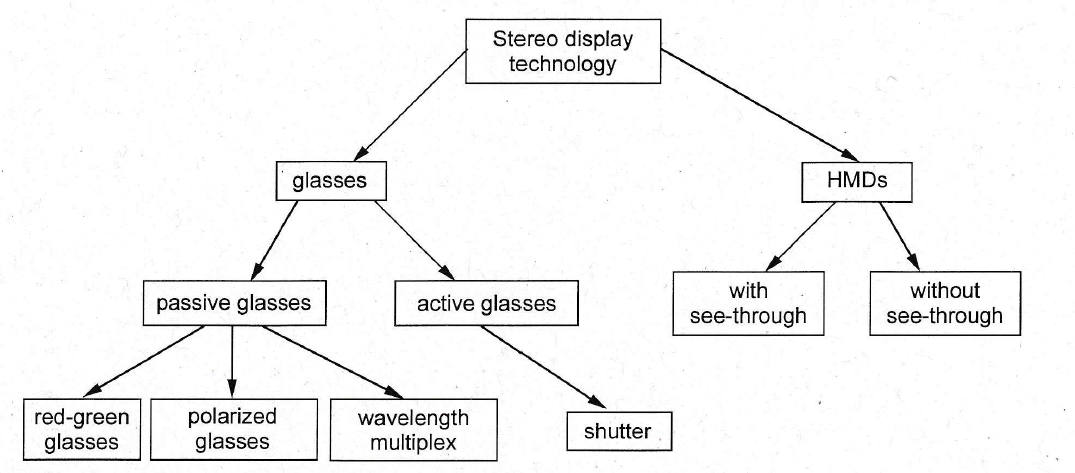
\includegraphics[scale=0.5]{5_103}
	
	\item Passive Red-Green Glasses (Anaglyphe Technology)
	\begin{itemize}
		\item Visualization devices produce two images, projected at the same time in red and green
		\item The two images are almost identical but slightly displaced towards each other by the amount of the horizontal parallax(eye distance)
		\item The image is viewed through filters, red filter in front of one eye and green filter in front if the other(with bare eyes the image appear blurred)
		\item Eyes see a slightly different image due to the parallax, resulting in a stereoscopic image
		\item Drawback: only red and green images can be generated, which appear monochrome when wearing the glasses \\
		if other colors are used the stereoscopic effect is destroyed
		\item Advantage: cheap installation of the system
	\end{itemize}

	\item Polarized Glasses (Linearly)
	\begin{itemize}
		\item A stereoscopic image with full colors can be generated since the polarization filters do not filter out any specific frequencies
		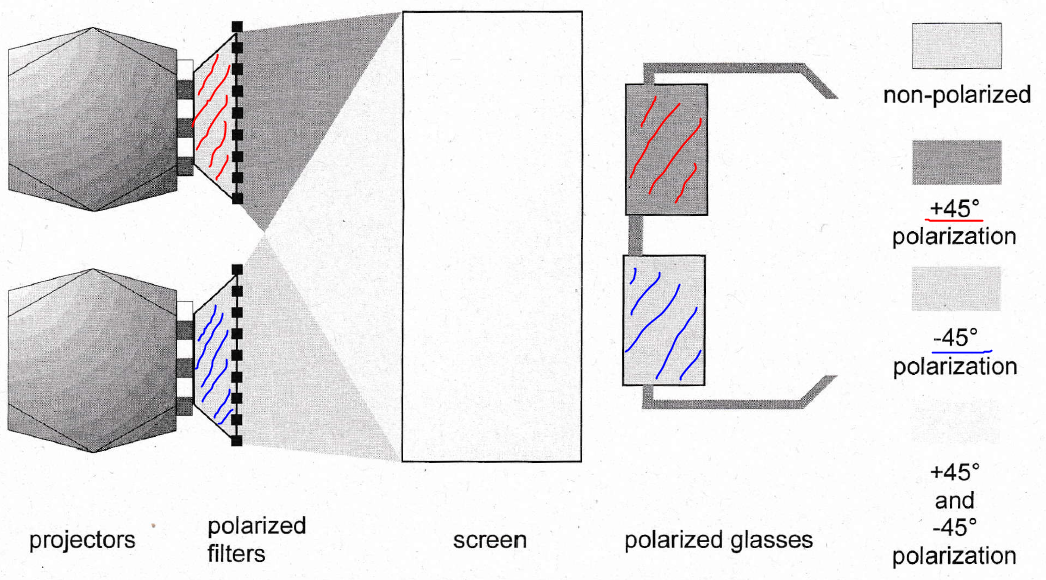
\includegraphics[scale=0.4]{5_106}
		\item Today, using only one projector is possible but with an additional polarization filter that can be electrically switched, "z-screen" \\
		however this results in a change from a parallel projection of the two required channels to a serial projection, which requires projectors that can switch fast enough
		\item Advantage: color images can be displayed \\
		Glasses have a low transmission loss and thus the images stay bright \\
		Moving pictures can be displayed with the maximum image repetition frequency available from the projectors \\
		Filters and glasses are inexpensive
		\item Drawback: two projectors(or one projector with a z-screen) are needed, as well as a specially coated screen that doesn't change the polarization between the incoming and the reflected light\\
		Linear polarization causes losses
		\begin{itemize}
			\item Transmittance of the polarization filter is defined as K and is between a maximum value k\textsubscript{2} and a minimum value  k\textsubscript{1}
			\item if a polarization filter is placed in front of a projector that emits unpolarized light: $ K = \frac{ k\textsubscript{2} + k\textsubscript{1}}{2} $
			\item two filters (projector and eye) polarized in the same direction: $ H\textsubscript{0} = \frac{ k\textsubscript{2}^2 + k\textsubscript{1}^2}{2} $
			\item if the orientations of the two filters are perpendicular to each other: $ H\textsubscript{90} = k\textsubscript{2}*k\textsubscript{1} $ \\
			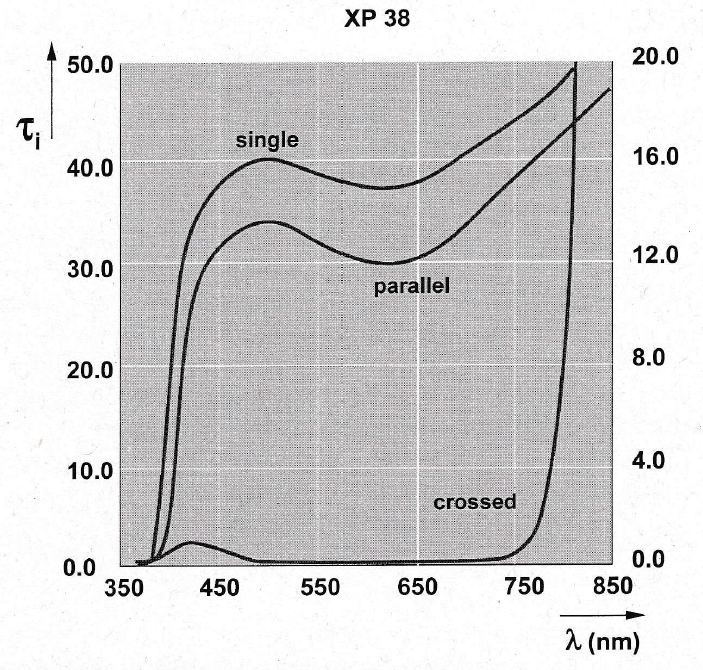
\includegraphics[scale=0.3]{5_108}
			\item the lower curve is also called "leakage"
			\item Problem: the alignment of the filters depends on the posture or on the head tipping of the audience; even small rotations of the head lead to a significantly increased leakage or crosstalk(sometimes called ghosting) \\
			relationship between the angle $\theta$ and the transmittance: $ K = (k\textsubscript{1}-k\textsubscript{2})*\cos ^2(\theta)+k\textsubscript{2} $ \\
		\end{itemize}
	\end{itemize}
	
	\item Polarized Glasses (Circular)
	\begin{itemize}
		\item The superposition of two linearly polarized waves, which are orthogonal to each other and which have a phase shift of 90$^{\circ}$, results in a circularly polarized wave
		\item If two sinusoidal oscillations with the same amplitude are superimposed, the E-vector does not oscillate anymore within the plane, but rotates around the z-axis \\
		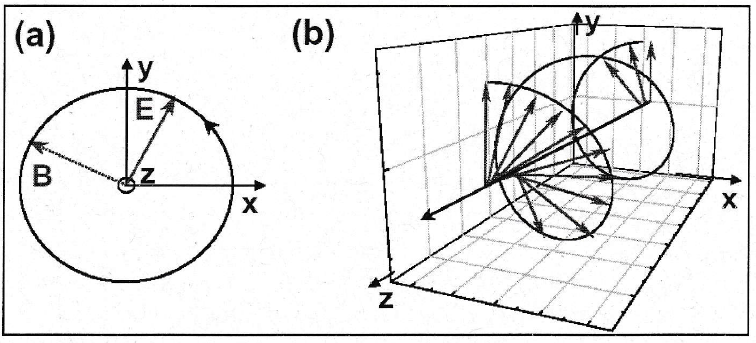
\includegraphics[scale=0.5]{5_112}
		\item The set-up for generating circularly polarized light consists of a filter for linear polarization and a quarter-wavelength retarder \\
		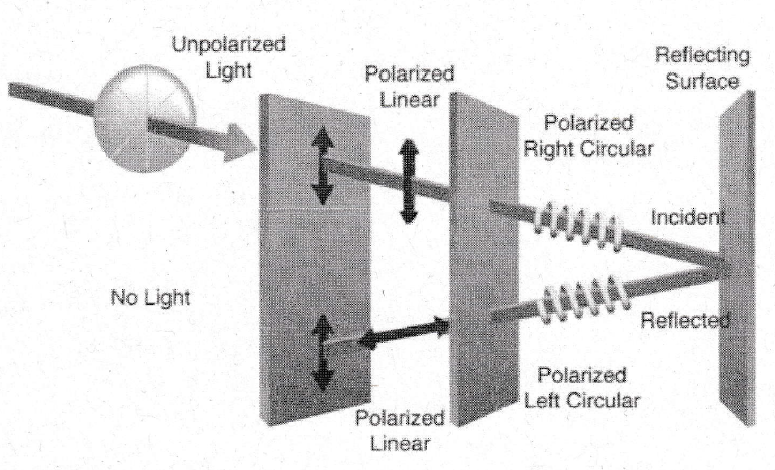
\includegraphics[scale=0.5]{5_113}
		\item Retarder: to transform linearly polarized light into circularly polarized light) \\
		consists of a material that retards the incoming light depending on the polarization due to multiple reflections in the material \\
		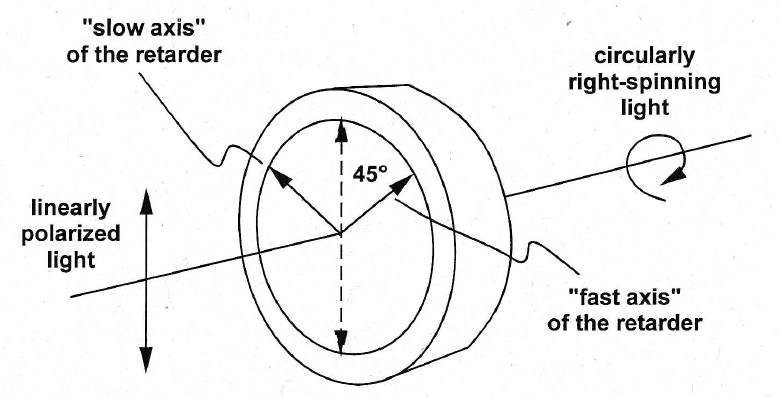
\includegraphics[scale=0.4]{5_114}
		\item The linear polarization of the incoming light has an angle of 45$^{\circ}$ to the slow axis and to the fast axis as well and is thus divided into two identical parts. Between the fast and the slow axis, there is a runtime difference of $\frac{\lambda}{4}$ for a given wavelength. The superposition of both light paths gives the wanted circular polarization
		\item The wave changes its spin orientation and reaches the user by the reflection on the screen. The
user wears glasses with another retarder and a polarization filter. The retarder converts the circularly polarized light into light with linear polarization.
	\end{itemize}
	
	\item Shutter Glasses
	\begin{itemize}
		\item The image on the visual output device is changed periodically, and an image for the left and the right eye is displayed alternately(two images are slightly different from each other due to the eye distance)
		\item The user wears shutter glasses, which are synchronized with the displayed images and alternately darken the left and the right eye
		\item Thus, every eye has a certain perspective and the stereoscopic sensation arises
		\item An infrared emitter sends synchronization pulses to the glasses which work with the typical LC-principle
		\item Advantage: low cost of the overall system
		\item Drawback: the user has to turn his head towards the monitor or the screen all the time(because otherwise infrared link cannot synchronize) \\
		the active shutter glasses are rather expensive
		\item When displaying active stereo images on normal TV sets, the even lines are used for the left eye while the odd lines are used for the right eye
	\end{itemize}
	
	\item Head Mounted Display (HMD)
	\begin{itemize}
		\item The idea of HMD is based on a stereoscope
		\item Advantage: the natural head movements are not restricted, so the user can freely explore by moving around and watching from different positions
		\item Drawback: heavy weight of the device, relatively small field of view(FOV)
		\item In order to address the two displays of an HMD, typically two graphics cards are needed but also possible to use only one graphics card by applying 'field-sequential procedure' or 'interlaced procedure' \\
		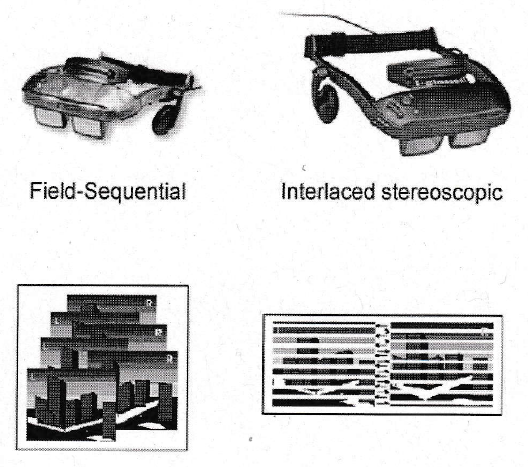
\includegraphics[scale=0.6]{5_120}
		\item Field-sequential procedure reduces the image repetition frequency by half, Interlaced procedure reduces the image resolution by half
		\item Angular resolution is one way to compare the perceived image quality \\
		takes 2 factors into account:
		\begin{itemize}
			\item The horizontal and vertical resolution of the internal display system(CRT or
LCD) in pixels
			\item The horizontal field of view(FOV) in degrees
		\end{itemize}
		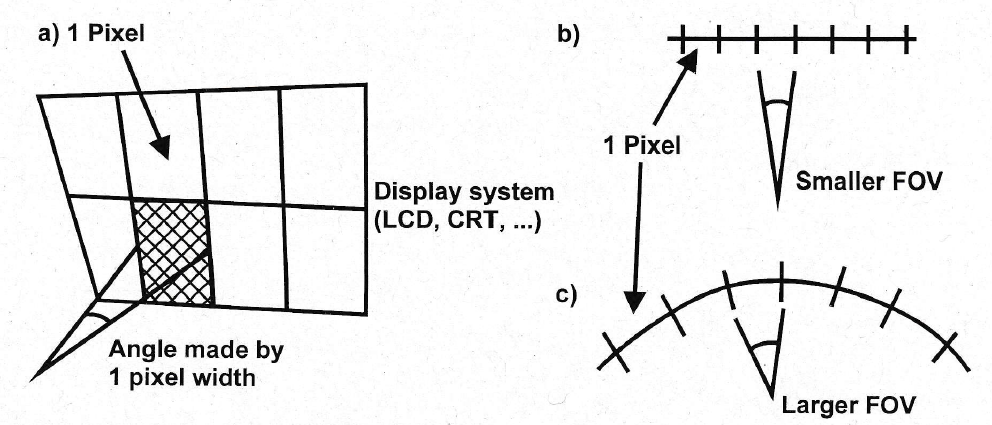
\includegraphics[scale=0.4]{5_121}
		\item FOV is hard to measure since there exists no standard method \\
		the main reason for the large variations is that some HMDs only allow a monoscopic display while others allow a stereoscopic vision(In case of a stereoscopic vision, the two displays must overlap which means FOV is limited and could be very small)
		\item Even though 20 percent of FOV being the central stereopsis region(overlap) is sufficient to give the user a good sense of depth, the overlap region is set to a greater value to provide a safety margin in case the user's gaze changes; the regions of overlap are very different depending on the devices
	\end{itemize}
	
	\item 3D Displays, Autostereoscopic Displays
	\begin{itemize}
		\item For autostereoscopic displays, the user don't have to wear special devices
		\item In principle, autostereoscopic displays are split into projective and volumetric procedures
		\item Parallax Barriers: a vertical grid of one pixel in width, which generates small barriers that block the view onto the display behind \\
		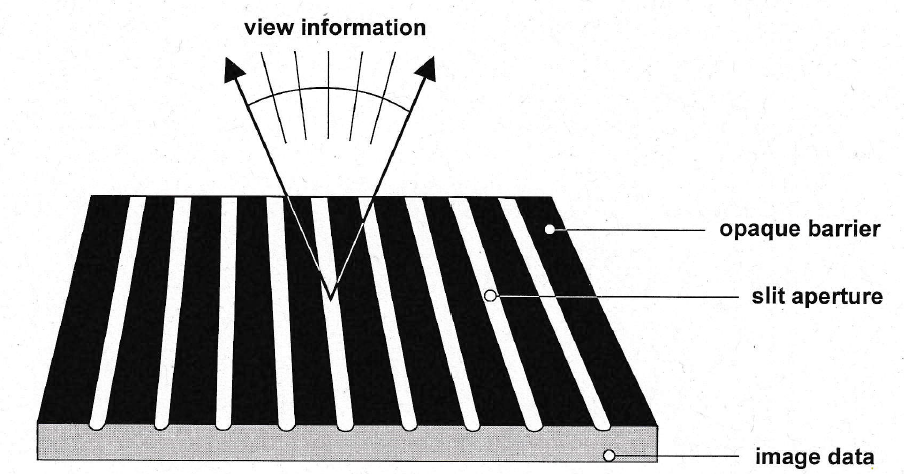
\includegraphics[scale=0.4]{5_126} \\
		Due to the small size of the blanked pixel columns, the visible system does not recognize the mask and generates a three-dimensional scene out of the two perceived images \\
		This procedure can also be used for the generation of more than two independent views by varying the distance and the width of the parallax barriers
		\item Lenticular Lenses: a layer of vertical semi-cylindrical lenses can be used to display adjacent pixels separately and to project them into the room \\
		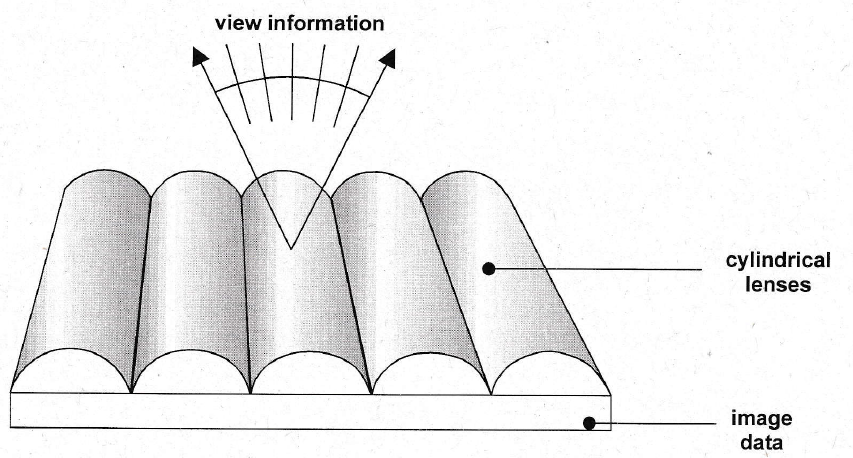
\includegraphics[scale=0.3]{5_127} 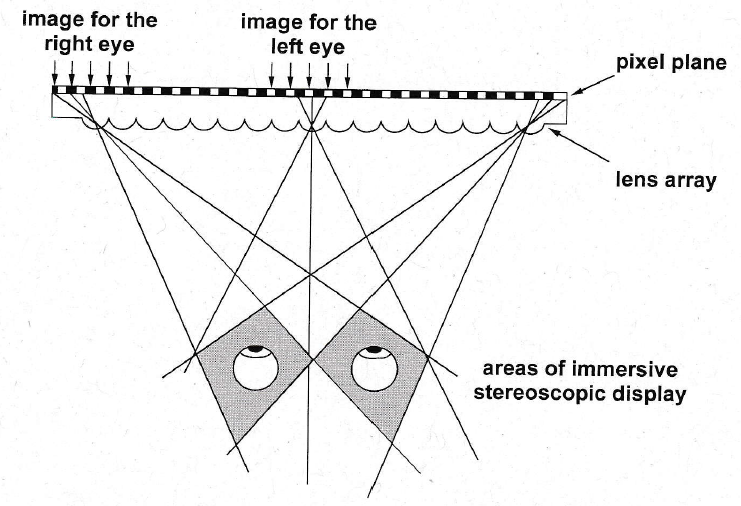
\includegraphics[scale=0.3]{5_128}\\
		very similar to the method of parallax barriers, but the lenticular lenses do not allow any direct view onto the pixels of the LC-display; only the amount of light is visible to the user that is refracted in direction of the actual eye position \\
		The lens array consists of a glass pane with a large amount of micro lenses \\
		Behind the lens array, two stereoscopic semi-images are displayed(odd columns for the right eye and even columns for the left eye); the computer has to generate two different signals for the displays, which will be combined by a multiplexer in an alternating way \\
		The stereoscopic sensation depends on the head position of the user, so the 3D display systems have an automatic adjusting system which adapts the monitor to the head movements \\
		A video camera takes an image of the user's eye distance, making it possible to readjust the position of the lens array \\
		Drawback: the user has to be at an exactly defined position(but multiple users are possible)
		\item Integral Imaging: expand the line-based idea to the vertical direction, an array of hemispheric lenses results instead of lenticular lenses \\
		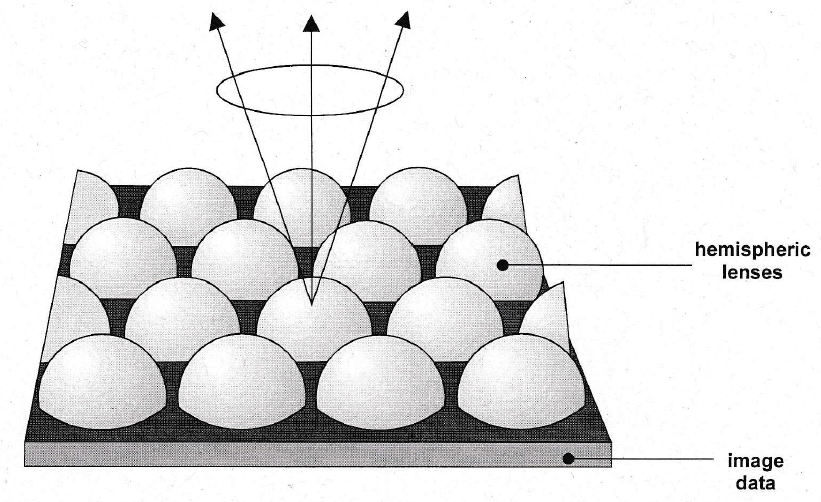
\includegraphics[scale=0.4]{5_131} \\
		The so-called "integral imaging" was firstly used with high-resolution images and allowed stereo- and motion parallaxes into all directions within a certain range
		\item Volumetric Displays: \\
		Volumetric procedures distinguish from the projective procedures by the way points in space are addressed; while the projective displays only throw pre-calculated perspective images into space, volumetric displays directly define each pixel within the projection volume with regard to its intensity and color \\
		e.g. Actuality Systems: a laminated helix rotates inside a glass sphere with such a high rotation speed that the helix becomes almost invisible. The required pixels in space are illuminated by three color lasers at that moment, when the surface of the helix is at the right location(below left) \\
		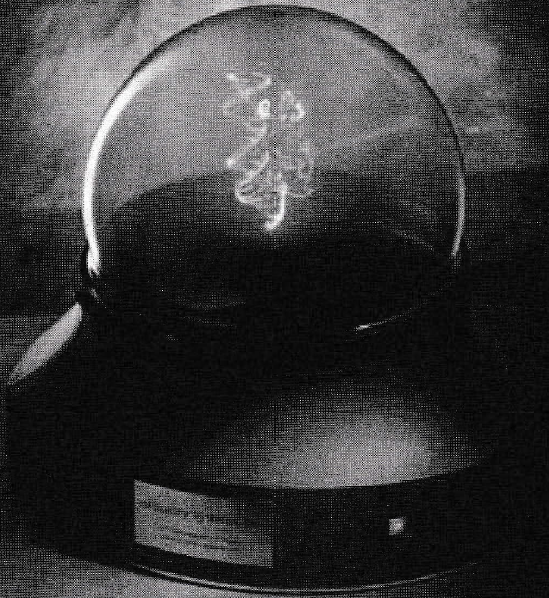
\includegraphics[scale=0.3]{5_133} 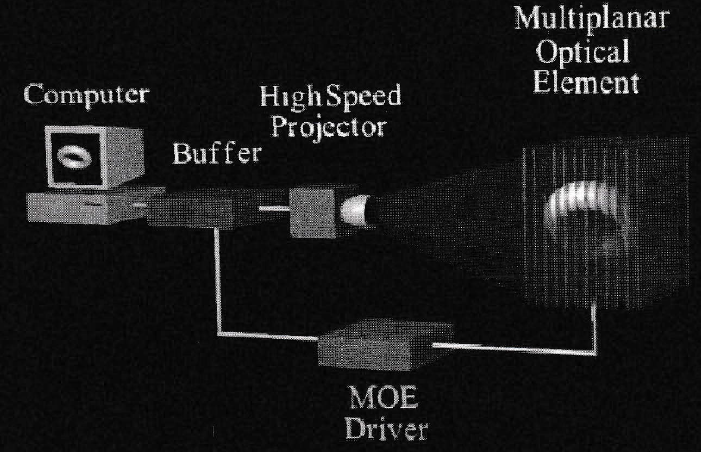
\includegraphics[scale=0.4]{5_134}
		\item DepthCube: a computer monitor that is based on a back projection system \\
		two main components: a high-speed video projector and a multiplanar optical element, in which
each slide defines a certain depth \\
		all pixels are really projected onto different locations in the projection space; the user has an impression of depth by accommodation and by convergence as well
	\end{itemize}
	
	\item Wavelength Multiplex Systems "Infitec"
	\begin{itemize}
		\item The perception of visible information is performed by receptors, which have different sensitivities to different colors
		\item It uses the fact that image information can be transmitted in parallel in slightly different wavelength triples(color values). The complete image information is split into two channels by this color separation \\
		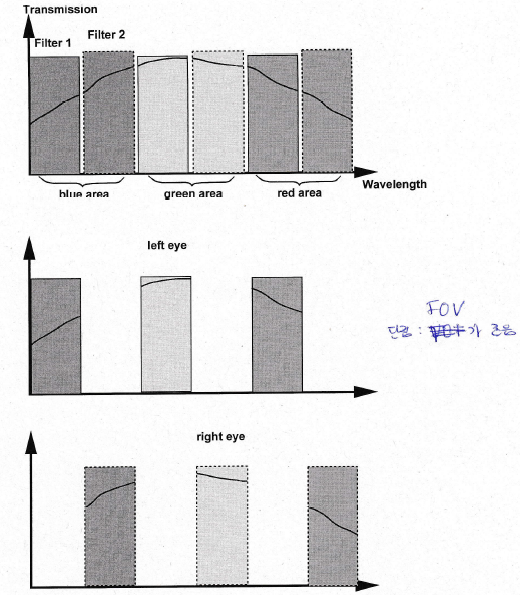
\includegraphics[scale=0.7]{5_136}
		\item Two projectors are required, each of them equipped with a special filter to perform a specific color shift
		\item Optical notch filters(realized by multi-layer dielectric coating onto a suitable carrier material) are needed to separate the content for left and right eye
		\item By increasing the amount of resonators in the optical notch filters, the quality and selectivity of the filter can be increased which determines the amount of parallel channels for transmitting the image content
		\item Advantage: a complete RGB-system per eye is available \\
		exists a possibility for simultaneous visualization of multiple, stereoscopic perspectives for more than one user \\
		the projection can also be performed in rooms with ambient light without any loss in contrast since the separation of different images is done by filters that have a very small optical bandwidth
		\item Constraint: all spectral frequencies are within the bandwidth of activation for one certain color receptor
	\end{itemize}		
	
\end{itemize}

\end{document}